\documentclass[border=6pt,tikz]{standalone}
\usepackage{tikz}
\usepackage{amsmath,amssymb}
\usetikzlibrary{arrows.meta,positioning,fit,backgrounds,calc,shapes.geometric,decorations.pathreplacing,patterns}
\definecolor{ink}{HTML}{1B2430}
\definecolor{muted}{HTML}{6B7785}
\definecolor{accent}{HTML}{2F6FB5}
\definecolor{accent2}{HTML}{C1611F}
\definecolor{good}{HTML}{2E7D5B}
\definecolor{soft}{HTML}{EDF2F7}
\definecolor{soft2}{HTML}{FBEDE2}
\definecolor{soft3}{HTML}{E6F0E9}
\tikzset{
  box/.style={draw=ink,line width=.7pt,rounded corners=2pt,fill=soft,inner sep=4pt,align=center,font=\sffamily\small},
  boxa/.style={box,fill=soft2},
  boxb/.style={box,fill=soft3},
  plain/.style={align=center,font=\sffamily\small,text=ink},
  tiny/.style={align=center,font=\sffamily\scriptsize,text=muted},
  ar/.style={-{Stealth[length=2.4mm]},draw=ink,line width=.7pt},
  arm/.style={-{Stealth[length=2.4mm]},draw=muted,line width=.6pt,dashed},
  nd/.style={circle,draw=ink,line width=.7pt,fill=white,minimum size=7mm,inner sep=0pt,font=\sffamily\scriptsize},
  ndf/.style={nd,fill=soft},
  ndt/.style={nd,fill=soft2},
}

\begin{document}
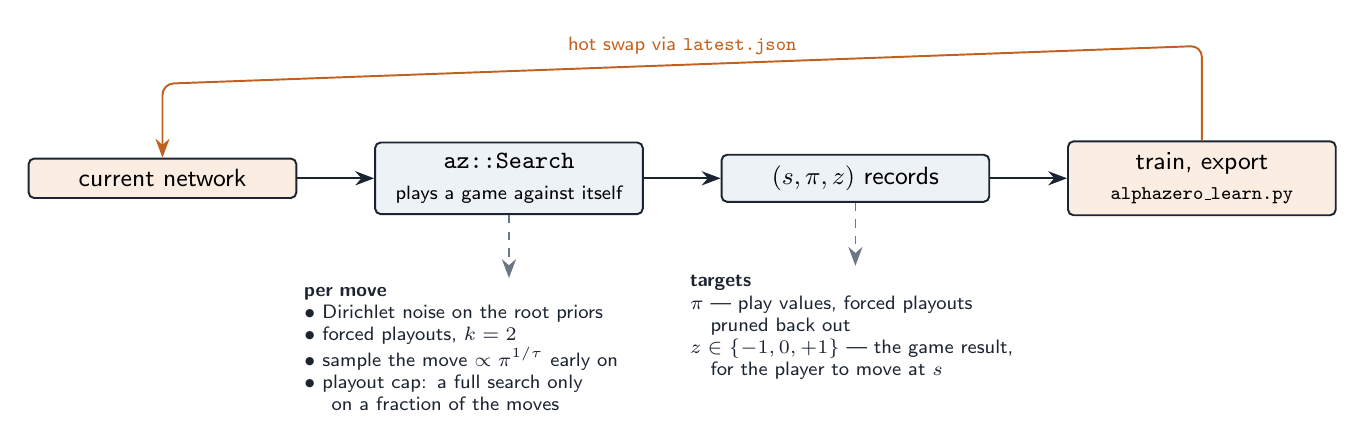
\begin{tikzpicture}[x=1mm,y=1mm]
  \node[boxa,minimum width=34mm] (net) at (0,0) {current network};
  \node[box,minimum width=34mm] (play) at (44,0) {\texttt{az::Search}\\\scriptsize plays a game against itself};
  \node[box,minimum width=34mm] (data) at (88,0) {$(s,\pi,z)$ records};
  \node[boxa,minimum width=34mm] (train) at (132,0) {train, export\\\scriptsize \texttt{alphazero\_learn.py}};
  \draw[ar] (net)--(play); \draw[ar] (play)--(data); \draw[ar] (data)--(train);
  \draw[ar,draw=accent2,rounded corners] (train.north) -- ++(0,12) -- node[tiny,above,text=accent2]{hot swap via \texttt{latest.json}} (0,12) -- (net.north);

  \node[tiny,below=8mm of play,text width=52mm,text=ink,align=left] (n1)
    {\textbf{per move}\\
     $\bullet$ Dirichlet noise on the root priors\\
     $\bullet$ forced playouts, $k=2$\\
     $\bullet$ sample the move $\propto \pi^{1/\tau}$ early on\\
     $\bullet$ playout cap: a full search only\\ \ \ \ \ on a fraction of the moves};
  \node[tiny,below=8mm of data,text width=42mm,text=ink,align=left] (n2)
    {\textbf{targets}\\
     $\pi$ --- play values, forced playouts\\ \ \ \ pruned back out\\
     $z\in\{-1,0,+1\}$ --- the game result,\\ \ \ \ for the player to move at $s$};
  \draw[arm] (play) -- (n1); \draw[arm] (data) -- (n2);
\end{tikzpicture}
\end{document}
